\documentclass[border=3mm,tikz,preview]{standalone}
\usepackage[utf8]{inputenc}
\usepackage{amsmath,amssymb,amsfonts}
\usepackage{graphicx}
\usepackage{tikz}
\usetikzlibrary{shapes.geometric, arrows.meta, positioning, shadows, calc, fit, backgrounds}
\usepackage{xcolor}
\begin{document}

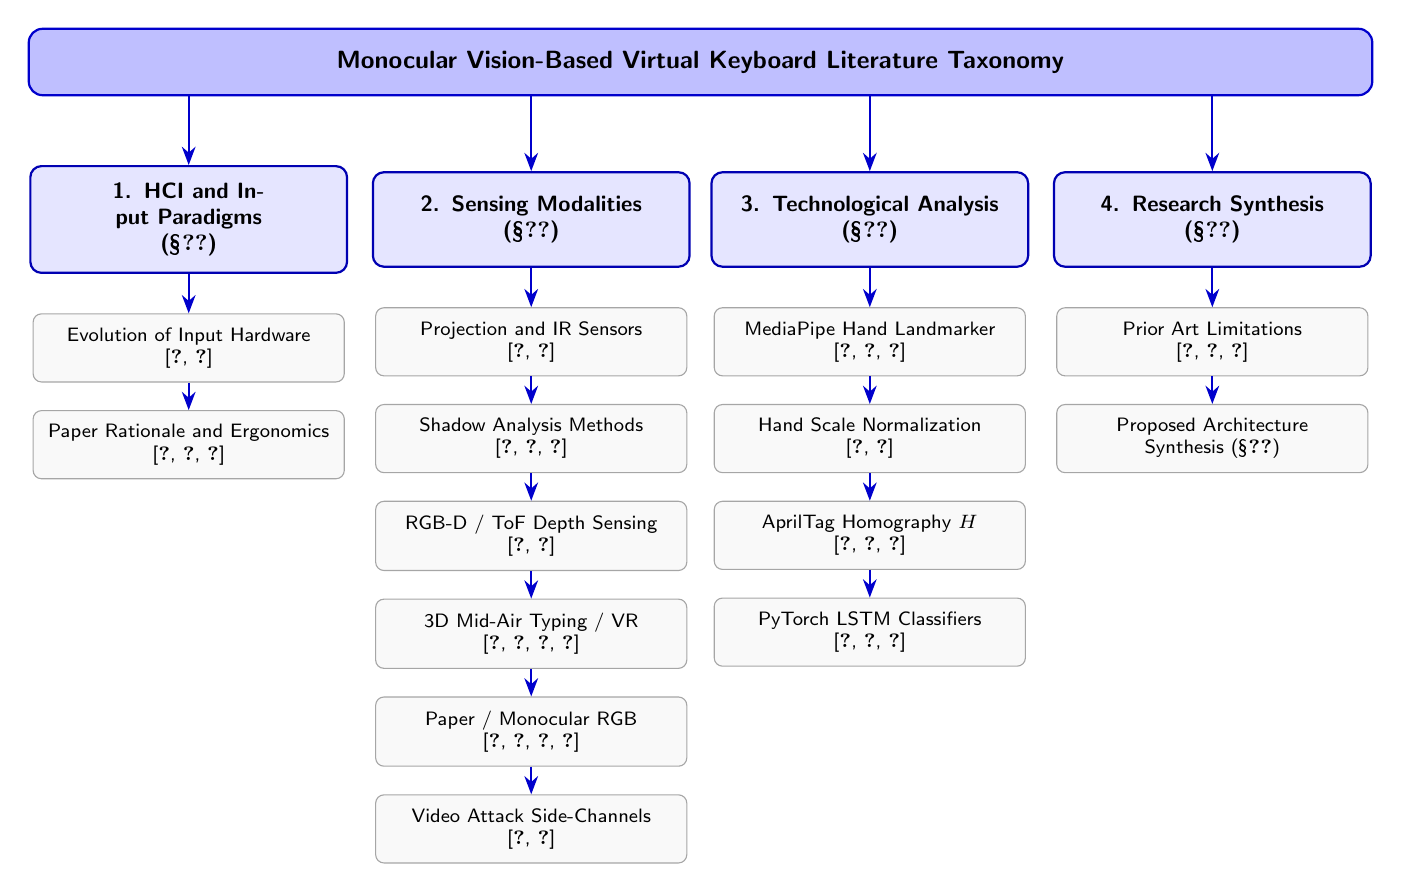
\begin{tikzpicture}[
    header/.style = {rectangle, draw=blue!80!black, fill=blue!25!white, thick, rounded corners=5pt, align=center, font=\sffamily\bfseries\small, inner sep=8pt, text width=16.5cm},
    box/.style = {rectangle, draw=blue!70!black, fill=blue!10!white, thick, rounded corners=4pt, align=center, font=\sffamily\bfseries\footnotesize, inner sep=6pt, text width=3.6cm, minimum height=1.2cm},
    subbox/.style = {rectangle, draw=gray!70, fill=gray!5!white, rounded corners=3pt, align=center, font=\sffamily\scriptsize, inner sep=5pt, text width=3.6cm},
    arrow/.style = {draw=blue!80!black, ->, >=Stealth, thick}
]

% Root Node
\node (root) [header, at={(0, 0)}] {\textbf{Monocular Vision-Based Virtual Keyboard Literature Taxonomy}};

% Level 1 Nodes - Perfectly leveled at y = -2.0cm across 4 distinct columns
\node (l1_domain) [box, at={(-6.5, -2.0)}] {1. HCI and Input Paradigms\\(\S\ref{sec:lit_domain_overview})};
\node (l1_systems) [box, at={(-2.15, -2.0)}] {2. Sensing Modalities\\(\S\ref{sec:lit_existing_systems})};
\node (l1_tech) [box, at={(2.15, -2.0)}] {3. Technological Analysis\\(\S\ref{sec:lit_technological_analysis})};
\node (l1_reflect) [box, at={(6.5, -2.0)}] {4. Research Synthesis\\(\S\ref{sec:lit_reflection})};

% Connections to Level 1
\draw [arrow] (root.south -| l1_domain.north) -- (l1_domain.north);
\draw [arrow] (root.south -| l1_systems.north) -- (l1_systems.north);
\draw [arrow] (root.south -| l1_tech.north) -- (l1_tech.north);
\draw [arrow] (root.south -| l1_reflect.north) -- (l1_reflect.north);

% Column 1: Domain Overview
\node (l2_history) [subbox, below=0.5cm of l1_domain] {Evolution of Input Hardware\\\cite{ReviewVirtualKeyboard2020, Lee2022Virtual}};
\node (l2_drivers) [subbox, below=0.35cm of l2_history] {Paper Rationale and Ergonomics\\\cite{Zhang2001Visual, Srivastava2012RealTime, Khare2019QWERTY}};

% Column 2: Existing Systems
\node (l2_proj) [subbox, below=0.5cm of l1_systems] {Projection and IR Sensors\\\cite{Cheng2015Fingertip, Kudale2016RealTime}};
\node (l2_shadow) [subbox, below=0.35cm of l2_proj] {Shadow Analysis Methods\\\cite{Thomas2013Camera, Posner2012Single, Yue2014Blind}};
\node (l2_depth) [subbox, below=0.35cm of l2_shadow] {RGB-D / ToF Depth Sensing\\\cite{Lee2019Virtual, Toshpulatov2024RealTime}};
\node (l2_air) [subbox, below=0.35cm of l2_depth] {3D Mid-Air Typing / VR\\\cite{Boletsis2019TextInput, Enkhbat2020HandKey, Lee2022Virtual, Yoo2026WordLevel}};
\node (l2_paper) [subbox, below=0.35cm of l2_air] {Paper / Monocular RGB\\\cite{Zhang2001Visual, Srivastava2012RealTime, Khare2019QWERTY, Maman2023TypeNet}};
\node (l2_attack) [subbox, below=0.35cm of l2_paper] {Video Attack Side-Channels\\\cite{Yue2014Blind, Yang2022Towards}};

% Column 3: Technological Analysis
\node (l2_pose) [subbox, below=0.5cm of l1_tech] {MediaPipe Hand Landmarker\\\cite{Zhang2020MediaPipe, GilMartin2023Hand, Andriyanov2025Improving}};
\node (l2_scale) [subbox, below=0.35cm of l2_pose] {Hand Scale Normalization\\\cite{Doan2022Efficient, Kumar2026Hybrid}};
\node (l2_fiducial) [subbox, below=0.35cm of l2_scale] {AprilTag Homography $H$\\\cite{Wang2016AprilTag2, Kallwies2020Determining, Pirchheim2011Homography}};
\node (l2_deep) [subbox, below=0.35cm of l2_fiducial] {PyTorch LSTM Classifiers\\\cite{Hochreiter1997LSTM, Nunez2018Convolutional, Gammulle2021TMMF}};

% Column 4: Research Synthesis
\node (l2_gap) [subbox, below=0.5cm of l1_reflect] {Prior Art Limitations\\\cite{Thomas2013Camera, Lee2019Virtual, Maman2023TypeNet}};
\node (l2_solution) [subbox, below=0.35cm of l2_gap] {Proposed Architecture\\Synthesis (\S\ref{sec:lit_reflection})};

% Vertical Column Connections
\draw [arrow] (l1_domain) -- (l2_history);
\draw [arrow] (l2_history) -- (l2_drivers);

\draw [arrow] (l1_systems) -- (l2_proj);
\draw [arrow] (l2_proj) -- (l2_shadow);
\draw [arrow] (l2_shadow) -- (l2_depth);
\draw [arrow] (l2_depth) -- (l2_air);
\draw [arrow] (l2_air) -- (l2_paper);
\draw [arrow] (l2_paper) -- (l2_attack);

\draw [arrow] (l1_tech) -- (l2_pose);
\draw [arrow] (l2_pose) -- (l2_scale);
\draw [arrow] (l2_scale) -- (l2_fiducial);
\draw [arrow] (l2_fiducial) -- (l2_deep);

\draw [arrow] (l1_reflect) -- (l2_gap);
\draw [arrow] (l2_gap) -- (l2_solution);

\end{tikzpicture}

\end{document}
